\documentclass{standalone}

\usepackage{amsmath,amsfonts,amssymb,amsthm,mathtools} 
\usepackage{fontspec}            % пакет для подгрузки шрифтов
\setmainfont{Amiri}   % задаёт основной шрифт документа

% why do we need \newfontfamily:
% http://tex.stackexchange.com/questions/91507/
\newfontfamily{\cyrillicfonttt}{Amiri}
\newfontfamily{\cyrillicfont}{Amiri}
\newfontfamily{\cyrillicfontsf}{Burst My Bubble}
% Иногда тех не видит структуры шрифтов. Эти трое бравых парней спасают ситуацию и доопределяют те куски, которые Тех не увидел.

\usepackage{unicode-math}     % пакет для установки математического шрифта
\setmathfont{Asana Math}      % шрифт для математики

\usepackage{polyglossia}      % Пакет, который позволяет подгружать русские буквы
\setdefaultlanguage{russian}  % Основной язык документа
\setotherlanguage{english}    % Второстепенный язык документа

\usepackage{pgf,tikz,pgfplots}
\usetikzlibrary{arrows,calc}
\usepackage{relsize} 

\usepackage{graphicx} 
\usepackage{rotating}
\usepackage{xcolor}
\usepackage{color}

\newcommand{\BBig}{\fontsize{60}{60}\selectfont}

\definecolor{bl}{HTML}{333333}
\definecolor{latxlatx}{HTML}{434545}


\begin{document}

\centering

\begin{tikzpicture}[scale=1]
\node[inner sep=0pt] (russell) at (14,0) {
\includegraphics[angle=0,scale=0.95]{pop2.jpg}}; 
\node[inner sep=0pt] (russell) at (0,0) {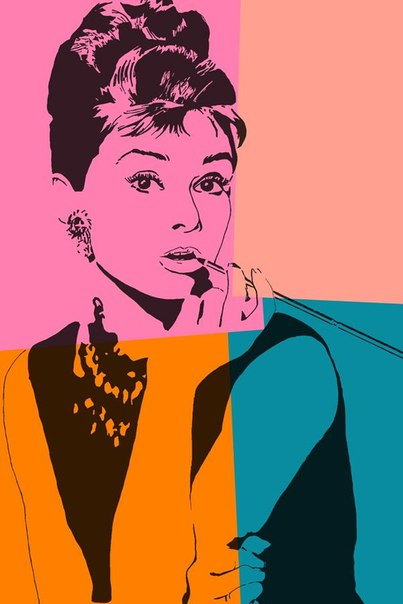
\includegraphics[angle=0,scale=1.312]{pop3.jpg}};    
\node[inner sep=0pt] (russell) at (-14.9,0) {
\includegraphics[angle=0,scale=1]{pop1.jpg}};   
\node[inner sep=0pt] (russell) at (-14.9,-20.4) {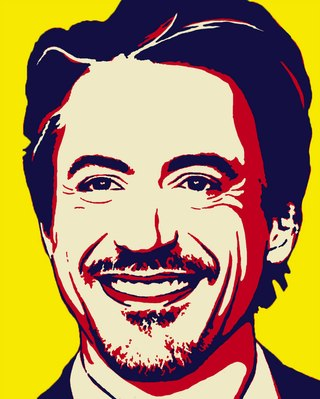
\includegraphics[angle=0,scale=1.4]{pop5.jpg}};   
\node[inner sep=0pt] (russell) at (0,-20) {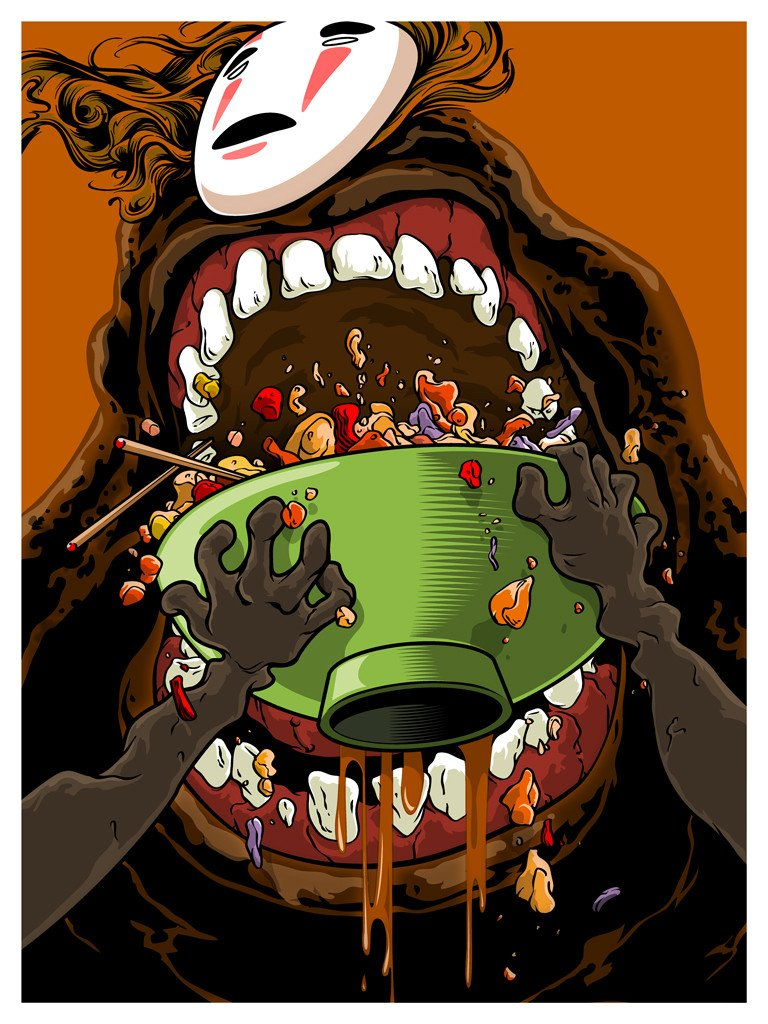
\includegraphics[angle=0,scale=0.88]{pop6.jpg}};   
\node[inner sep=0pt] (russell) at (14,-20) {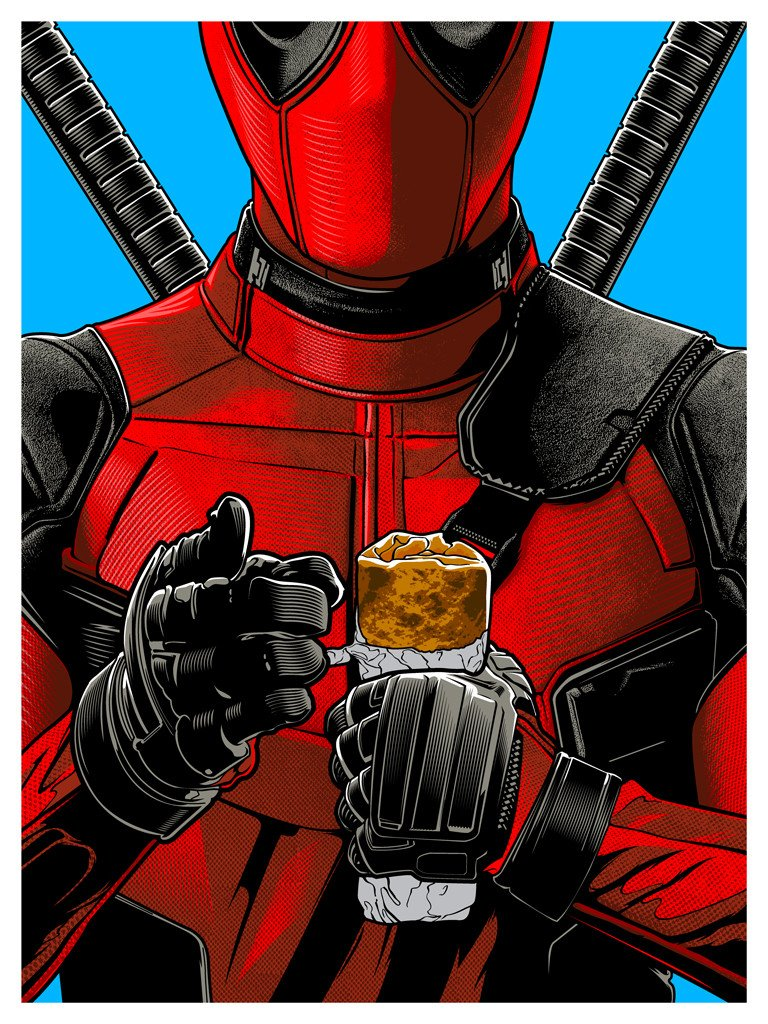
\includegraphics[angle=0,scale=4]{pop4.jpg}};   
\end{tikzpicture}

%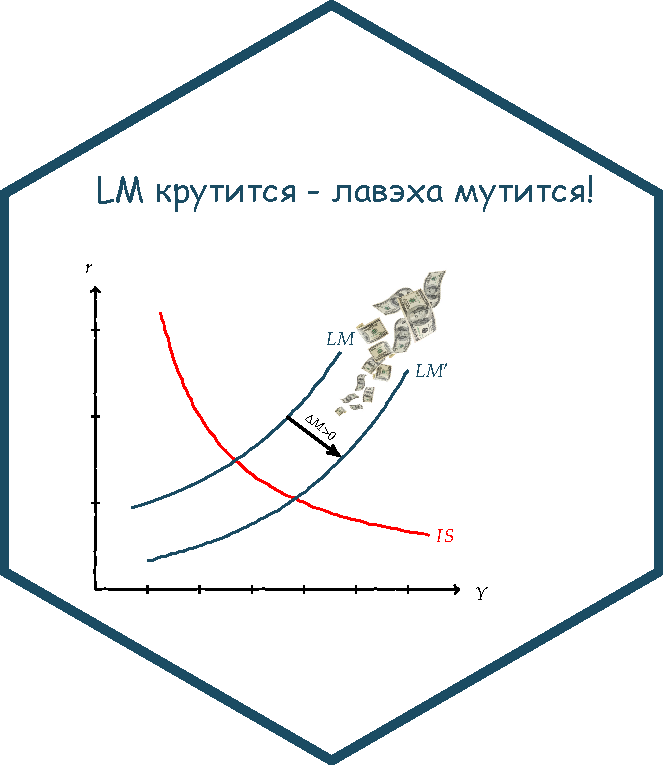
\includegraphics{ISLM.pdf}



\end{document}
